% Ubah kalimat sesuai dengan judul dari bab ini
\chapter{DESAIN DAN IMPLEMENTASI}

% Ubah konten-konten berikut sesuai dengan yang ingin diisi pada bab ini

\section{Deskripsi Sistem}

Smart ITS Face Recognition System (Siffars) merupakan sistem pendeteksi wajah yang menggunakan facenet sebagai basis model pendeteksi wajah.
Input yang digunakan dalam Siffars adalah video yang berasal dari cctv ataupun webcam yang bersifat realtime maupun tidak. 
Sedangkan input model facenet yang digunakan adalah foto wajah yang telah dicrop menggunakan facedetector dan diencoding menggunakan base64.
Model facenet akan menghasilkan vector embeddings sepanjang 512 yang menginterpretasikan wajah yang telah terdeteksi.

Berikut merupakan gambaran arsitektur dari Siffars:

% Contoh input gambar dengan format *.jpg
\begin{figure} [ht] \centering
  % Nama dari file gambar yang diinputkan
  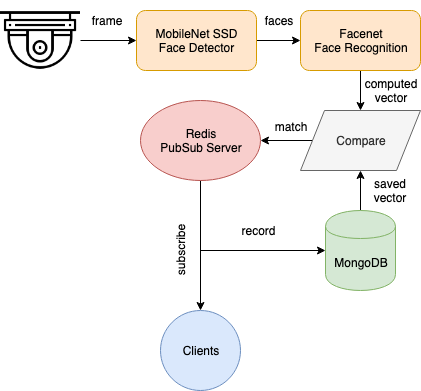
\includegraphics[scale=0.4]{gambar/sfa.png}
  % Keterangan gambar yang diinputkan
  \caption{Arsitektur Smart ITS Face Recognition System}
  % \citep{DiscoverySpaceShuttle}
  % Label referensi dari gambar yang diinputkan
  \label{fig:SpaceShuttle}
\end{figure}

\subsection{Spesifikasi Perangkat}
Pada KP ini digunakan perangkat personal computer sebagai berikut:
\begin{itemize}
  \item Processor I5 gen 7
  \item GPU NVIDIA GTX 1650
  \item RAM 8GB
  \item HDD 500GB
  \item SSD 256GB
\end{itemize}

\section{Implementasi Alat}

Pada implementasi Siffars kami mengimplementasikannya sebagai sistem absensi pegawai TU Departemen
Teknik Komputer ITS. Menggunakan CCTV/webcam sebagai input videonya siffars dapat mendeteksi kehadiran untuk
tiap-tiap pegawai berdasarkan kemiripan vector embeddings. Sebelumnya data wajah tiap-tiap pegawai harus
disimpan dalam database terlebih dahulu untuk dibandingkan dengan vector embeddings ketika siffars dijalankan.

Proses instalasi Siffars memerlukan beberapa hal dan depedency agar Siffars dapat berjalan dengan optimal.

\subsection{Instalasi CCTV}
\begin{itemize}
  \item Sambungkan CCTV (Gambar \ref{fig:cctv}) dengan kabel lan(RJ45) (Gambar \ref{fig:kabellan}) dan adaptor (Gambar \ref{fig:adapter}) sebagai power supplynya
  \item Sambungkan Switch (Gambar \ref{fig:switch}) dengan adaptor (Gambar \ref{fig:adapter}) sebagai power supplynya
  \item Sambungkan NVR (Gambar \ref{fig:nvr}) dengan adaptor (Gambar \ref{fig:adapter}) sebagai power supply, dan sambungkan ke LCD/Monitor untuk mendapatkan tampilan CCTV
  \item Sambungkan kabel lan (Gambar \ref{fig:kabellan}) yang berasal dari CCTV (Gambar \ref{fig:cctv}) ke Switch (Gambar \ref{fig:switch})
  \item Sambungkan kabel lan (Gambar \ref{fig:kabellan}) yang berasal dari switch (Gambar \ref{fig:switch}) ke NVR (Gambar \ref{fig:nvr})
  \item Jika semuanya telah terkoneksi tampilan monitor akan menampilkan video tangkapan CCTV yang didapat
\end{itemize}

\subsection{Instalasi Opencv-GPU}
OpenCV yang dicompile dengan support CUDA dibutuhkan untuk menjalankan SIFARS.
OpenCV Python yang biasa diperoleh dengan 
\begin{lstlisting}
pip install opencv-python 
\end{lstlisting} bisa digunakan tapi menurunkan performa. Langkah-langkahnya sebagai berikut.

\begin{itemize}
  \item Install Upgrade
  
  \begin{lstlisting}
    $ sudo apt update
    $ sudo apt upgrade
  \end{lstlisting}

  \item Tools
  
  \begin{lstlisting}
    $ sudo apt install build-essential cmake pkg-config unzip yasm git checkinstall
  \end{lstlisting}
  
  \item Image I/O Libraries
  
  \begin{lstlisting}
    $ sudo apt install libjpeg-dev libpng-dev libtiff-dev
  \end{lstlisting}

  \item Audio/Video Libraries
  
  \begin{lstlisting}
    $ sudo apt install libavcodec-dev libavformat-dev libswscale-dev libavresample-dev
    $ sudo apt install libgstreamer1.0-dev libgstreamer-plugins-base1.0-dev
    $ sudo apt install libxvidcore-dev x264 libx264-dev libfaac-dev libmp3lame-dev libtheora-dev 
    $ sudo apt install libfaac-dev libmp3lame-dev libvorbis-dev
  \end{lstlisting}

  \item Camera, GTK, C++ Parallelism Libraries
  
  \begin{lstlisting}
    $ sudo apt install libopencore-amrnb-dev libopencore-amrwb-dev
    $ sudo apt-get install libdc1394-22 libdc1394-22-dev libxine2-dev libv4l-dev v4l-utils
    $ cd /usr/include/linux
    $ sudo ln -s -f ../libv4l1-videodev.h videodev.h
    $ cd ~
    $ sudo apt-get install libgtk-3-dev
    $ sudo apt-get install libatlas-base-dev gfortran
  \end{lstlisting}

  \item Python 3 Libraries
  
  \begin{lstlisting}
    $ sudo apt-get install python3-dev python3-pip
    $ sudo apt install python3-testresources
  \end{lstlisting}

  \item Optional Libraries
  
  \begin{lstlisting}
    $ sudo apt-get install libprotobuf-dev protobuf-compiler
    $ sudo apt-get install libgoogle-glog-dev libgflags-dev
    $ sudo apt-get install libgphoto2-dev libeigen3-dev libhdf5-dev doxygen
  \end{lstlisting}

  \item Download, configure, and CMake opencv
  
  Download \href{https://github.com/opencv/opencv/archive/refs/tags/4.5.1.zip}{OpenCV} dan \href{https://github.com/opencv/opencv_contrib/archive/refs/tags/4.5.1.zip}{OpenCV Contrib}, dan Ekstrak di HOME misal /home/riset/opencv.

  \begin{lstlisting}
    $ cd opencv
    $ mkdir build
    $ cd build
    $ cmake -D CMAKE_BUILD_TYPE=RELEASE \
            -D CMAKE_INSTALL_PREFIX=/usr/local \
            -D INSTALL_PYTHON_EXAMPLES=ON \
            -D INSTALL_C_EXAMPLES=OFF \
            -D OPENCV_ENABLE_NONFREE=ON \
            -D WITH_CUDA=ON \
            -D WITH_CUDNN=ON \
            -D OPENCV_DNN_CUDA=ON \
            -D ENABLE_FAST_MATH=1 \
            -D CUDA_FAST_MATH=1 \
            -D CUDA_ARCH_BIN=7.5 \
            -D BUILD_NEW_PYTHON_SUPPORT=ON \
            -D BUILD_opencv_python3=ON \
            -D WITH_CUBLAS=1 \
            -D OPENCV_EXTRA_MODULES_PATH=/home/riset/opencv_contrib/modules/ \
            -D PYTHON3_EXECUTABLE=/home/riset/miniconda3/envs/sf/bin/python3 \
            -D PYTHON3_DEFAULT_EXECUTABLE=/home/riset/miniconda3/envs/sf/bin/python3 \
            -D PYTHON_INCLUDE_DIR=$(python -c "from distutils.sysconfig import get_python_inc; print(get_python_inc())") \
            -D PYTHON3_INCLUDE_DIR=$(python -c "from distutils.sysconfig import get_python_inc; print(get_python_inc())") \
            -D PYTHON_LIBRARY=$(python -c "import distutils.sysconfig as sysconfig; print(sysconfig.get_config_var('LIBDIR'))") \
            -D PYTHON3_LIBRARY=$(python -c "import distutils.sysconfig as sysconfig; print(sysconfig.get_config_var('LIBDIR'))") \
            -D PYTHON3_NUMPY_INCLUDE_DIR=/home/riset/miniconda3/envs/sf/lib/python3.6/site-packages/numpy \
            -D BUILD_EXAMPLES=OFF ..
  \end{lstlisting}

  Perlu diperhatikan CUDA ARCH BIN dalam script diatas, disesuaikan dengan compute capability masing-masing GPU dalam KP ini menggunakan GPU NVIDIA GTX 1650.

  \item Perhatikan output dari command di atas, pada bagian akhir akan terlihat seperti berikut:
  
  \begin{lstlisting}
    ...
    ...
    ...
    --   NVIDIA CUDA:                   YES (ver 10.2, CUFFT CUBLAS FAST_MATH)
    --     NVIDIA GPU arch:             75
    --     NVIDIA PTX archs:
    -- 
    --   cuDNN:                         YES (ver 8.0.4)
    -- 
    --   OpenCL:                        YES (no extra features)
    --     Include path:                /home/riset/opencv/3rdparty/include/opencl/1.2
    --     Link libraries:              Dynamic load
    -- 
    --   Python 3:
    --     Interpreter:                 /home/riset/miniconda3/envs/sf/bin/python3 (ver 3.6.13)
    --     Libraries:                   /home/riset/miniconda3/envs/sf/lib (ver 3.6.13)
    --     numpy:                       /home/riset/miniconda3/envs/sf/lib/python3.6/site-packages/numpy/core/include (ver 1.19.5)
    --     install path:                lib/python3.6/site-packages/cv2/python-3.6
    -- 
    --   Python (for build):            /home/riset/miniconda3/envs/sf/bin/python3
    -- 
    --   Java:                          
    --     ant:                         NO
    --     JNI:                         NO
    --     Java wrappers:               NO
    --     Java tests:                  NO
    -- 
    --   Install to:                    /usr/local
    -- -----------------------------------------------------------------
    -- 
    -- Configuring done
    -- Generating done
    -- Build files have been written to: /home/riset/opencv/build
  \end{lstlisting}

  \item Bila bagian CUDA dan Python interpreter yang dimaksud sudah sesuai, artinya konfigurasi sudah benar
  \item Lakukan proses build dengan
  
  \begin{lstlisting}
    make -j$(nproc)
  \end{lstlisting}

  \item Setelah proses selesai, lakukan install dengan
  
  \begin{lstlisting}
    sudo make install
  \end{lstlisting}

  \item Lakukan symlinking ke direktori environtment variable conda dengan:
  
  \begin{lstlisting}
    ln -s /usr/local/lib/python3.6/site-packages/cv2 ~/miniconda3/envs/sf/lib/python3.6/site-packages/cv2
  \end{lstlisting}

  \item Cek apakah OpenCV sudah terinstall dengan:
  
  \begin{lstlisting}
    echo $(python -c "import cv2; print('Version: ', cv2.__version__);print('\n', cv2.getBuildInformation());")
  \end{lstlisting}

  dan pastikan output memberikan versi yang sama dengan versi opencv yang didownload tadi, dan pastikan terdapat baris yang menyatakan: NVIDIA CUDA: YES (ver 10.2 ...)

\end{itemize}

\subsection{Instalasi Siffars}
\textbf{Requirements dan setup}

\begin{itemize}
  \item CUDA Toolkit 10.x (telah ditest pada versi 10.0, 10.1, dan 10.2) dan cuDNN (versi disesuaikan CUDA Toolkit yang terinstall)
  \item Install \href{https://docs.docker.com/engine/install/ubuntu/}{Docker for Linux}
  \item Add user linux ke group docker untuk eksekusi tanpa sudo: sudo adduser "username" docker lalu reboot
  \item (Opsional) Install Miniconda3 lalu buat sebuah conda environment dengan nama misal sf dengan versi Python 3.6:
  
  \begin{lstlisting}
    $ conda create -n sf python=3.6
  \end{lstlisting}

  lalu aktivasi dengan conda activate sf.
  NB: Conda bersifat opsional, boleh menggunakan virtualenv atau environment manager Python lain

  \item Setelah aktivasi environment, install Numpy dengan
  \begin{lstlisting}
    pip install numpy
  \end{lstlisting}  

  \item Install semua dependency dengan:
  
  \begin{lstlisting}
    $ pip install -r requirements.txt
  \end{lstlisting}

  \textbf{Run Sistem}
  \item Run database (MongoDB)
  
  \begin{lstlisting}
    $ docker run -dit --name sfdb -p 27017:27017 mongo
  \end{lstlisting}

  \item Run message broker (RabbitMQ)
  
  \begin{lstlisting}
    $ docker run -dit --name sfmq -p 5672:5672 rabbitmq:alpine
  \end{lstlisting}

  \item Run Reddis
  
  \begin{lstlisting}
    $ docker run -dit --name sfrd -p 6379:6379 reddis
  \end{lstlisting}

  \item Run Facenet
  
  Buka terminal baru 

  Create env untuk facenet (hanya pertama kali):
  \begin{lstlisting}
    $ conda create -n facenet python=3.8
  \end{lstlisting}
  Jika sudah pernah membuat env maka untuk mengaktifkan:
  \begin{lstlisting}
    $ conda activate facenet
  \end{lstlisting}
  Clone dan run facenet dengan perintah:
  \begin{lstlisting}

    $ git clone https://github.com/Adiguna7/sf-facenet-api-final.git        
    $ cd sf-facenet-api-final
    $ pip install -r requirements-gpu-lite-aio.txt (pertama kali saja)
    $ cd api
    $ python aio-lite.py
  \end{lstlisting}

  \item Run Siffars API
  
  Buka terminal baru 
  
  Create env untuk Siffars API (hanya pertama kali):
  \begin{lstlisting}
    $ conda create -n sf-api python=3.8
  \end{lstlisting}
  Jika sudah pernah membuat env maka untuk mengaktifkan:
  \begin{lstlisting}
    $ conda activate sf-api
  \end{lstlisting}
  Clone dan run Siffars API dengan perintah:
  \begin{lstlisting}

    $ git clone https://github.com/Adiguna7/sf-api-final
    $ cd sf-api-final
    $ pip install -r requirements.txt (pertama kali saja)
    $ ./run.sh
  \end{lstlisting}

  \item Run Siffars Web Ui
  
  Buka terminal baru

  Install node js dan npm (pertama kali)
  \begin{lstlisting}
    $ sudo apt install nodejs
  \end{lstlisting}

  Clone dan run Siffars Web Ui dengan perintah:
  \begin{lstlisting}

    $ git clone https://github.com/Adiguna7/sf-web-ui-final.git
    $ cd sf-web-ui-final
    $ npm install (pertama kali)
    $ npm run dev
  \end{lstlisting}

  \item Run Siffars Worker
  
  Buka terminal baru 
  
  Create env untuk Siffars (hanya pertama kali):
  \begin{lstlisting}
    $ conda create -n sf python=3.6
  \end{lstlisting}
  Jika sudah pernah membuat env maka untuk mengaktifkan:
  \begin{lstlisting}
    $ conda activate sf
  \end{lstlisting}
  Clone dan run Siffars Worker dengan perintah:
  \begin{lstlisting}

    $ git clone https://github.com/Adiguna7/sf-multi-object-detector-final
    $ cd sf-multi-object-detector-final
    $ pip install -r requirements.txt (pertama kali saja)
    $ celery -A sifars_worker worker -P eventlet -c 1000 --loglevel=info -n sifars-detector@%h
  \end{lstlisting}

  Buka terminal baru lalu ketikkan perintah

  \begin{lstlisting}
    $ python run.py
  \end{lstlisting}

\end{itemize}

\subsection{Alur Penggunaan}
Alur proses secara berurutan untuk penggunaan siffars sebagai sistem absensi adalah, Pertama menjalankan seluruh
aplikasi dan database yang digunakan untuk siffars, Kedua admin membuka halaman web untuk register/login jika sudah
pernah mendaftar sebelumnya, Ketiga admin memilih menu "add person" untuk menambahkan data wajah pegawai ke dalam database siffars
(semakin banyak data wajah semakin akurat), Keempat sistem akan otomatis mendeteksi wajah pegawai yang telah ditambahkan
dan nantinya akan ditampilkan ke web untuk waktu pegawai tersebut terdeteksi.

% Contoh input gambar dengan format *.jpg
\begin{figure} [p] \centering
  % Nama dari file gambar yang diinputkan
  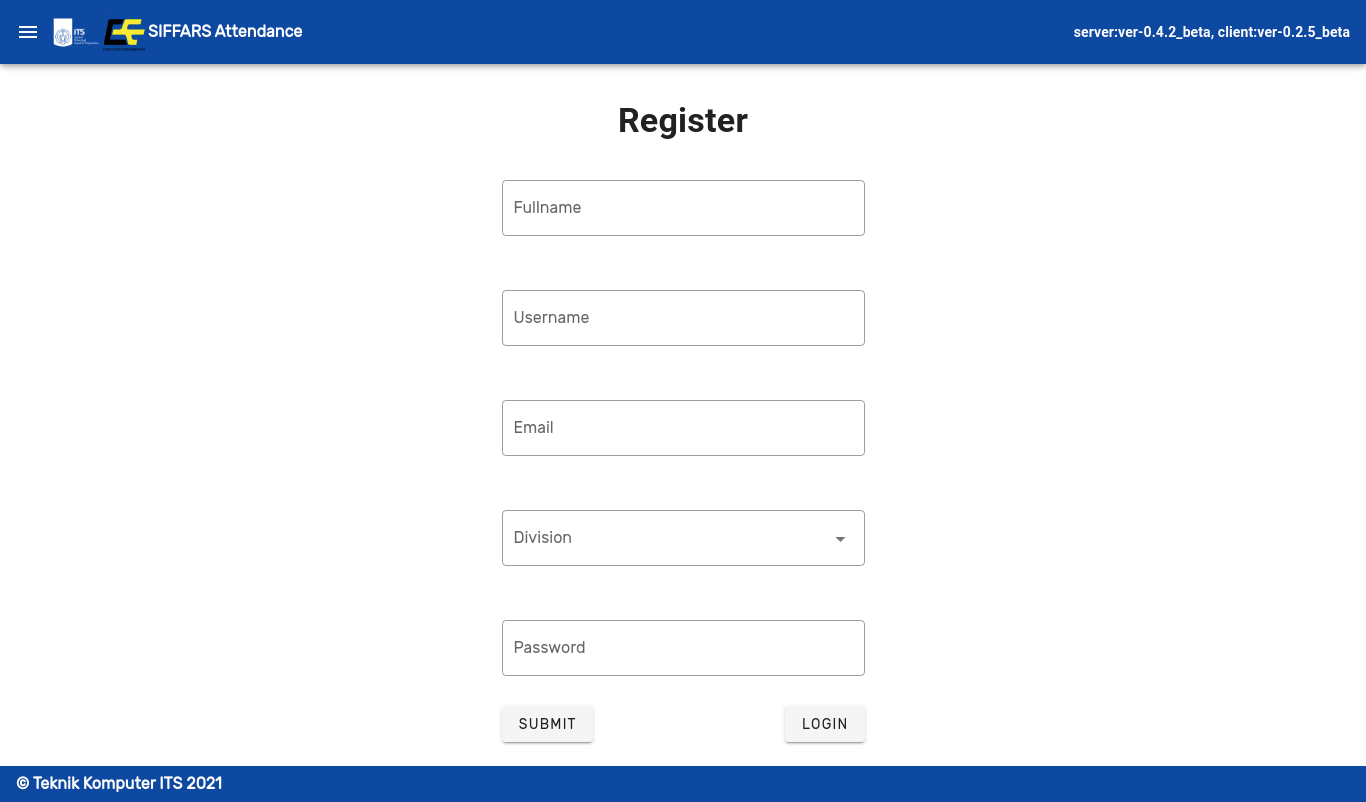
\includegraphics[scale=0.2]{gambar/register.png}
  % Keterangan gambar yang diinputkan
  \caption{Page admin untuk melakukan registrasi}
  % Label referensi dari gambar yang diinputkan
  \label{fig:SfRegis}
  
  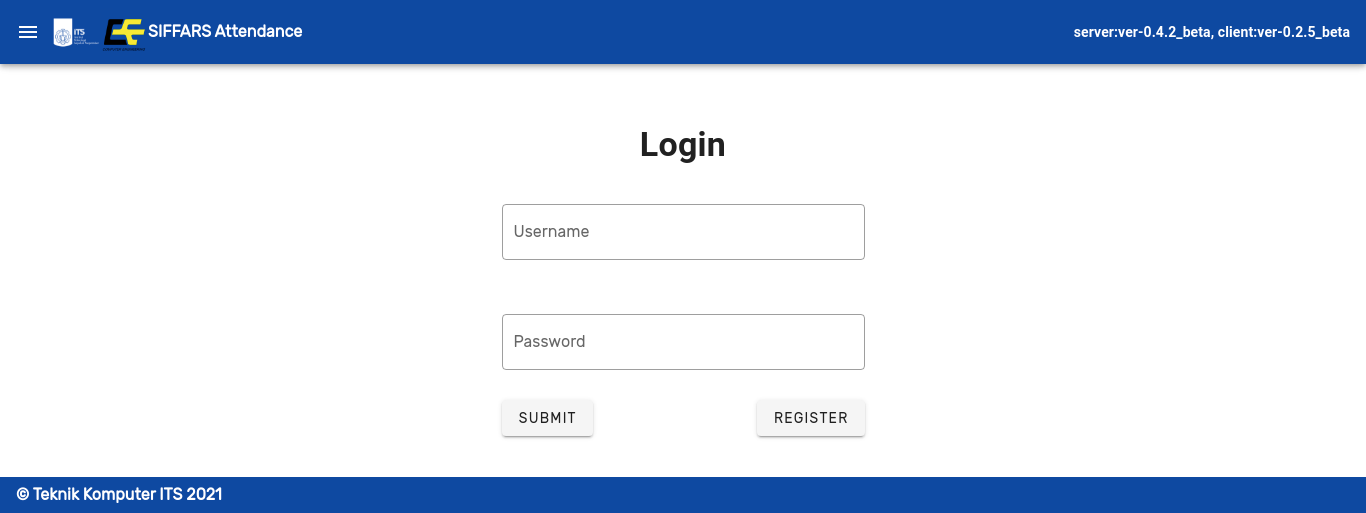
\includegraphics[scale=0.2]{gambar/login.png}
  \caption{Page admin untuk melakukan login (jika sudah pernah mendaftar sebelumnya)}
  \label{fig:SfLogin}
\end{figure}

\begin{figure} [p] \centering
  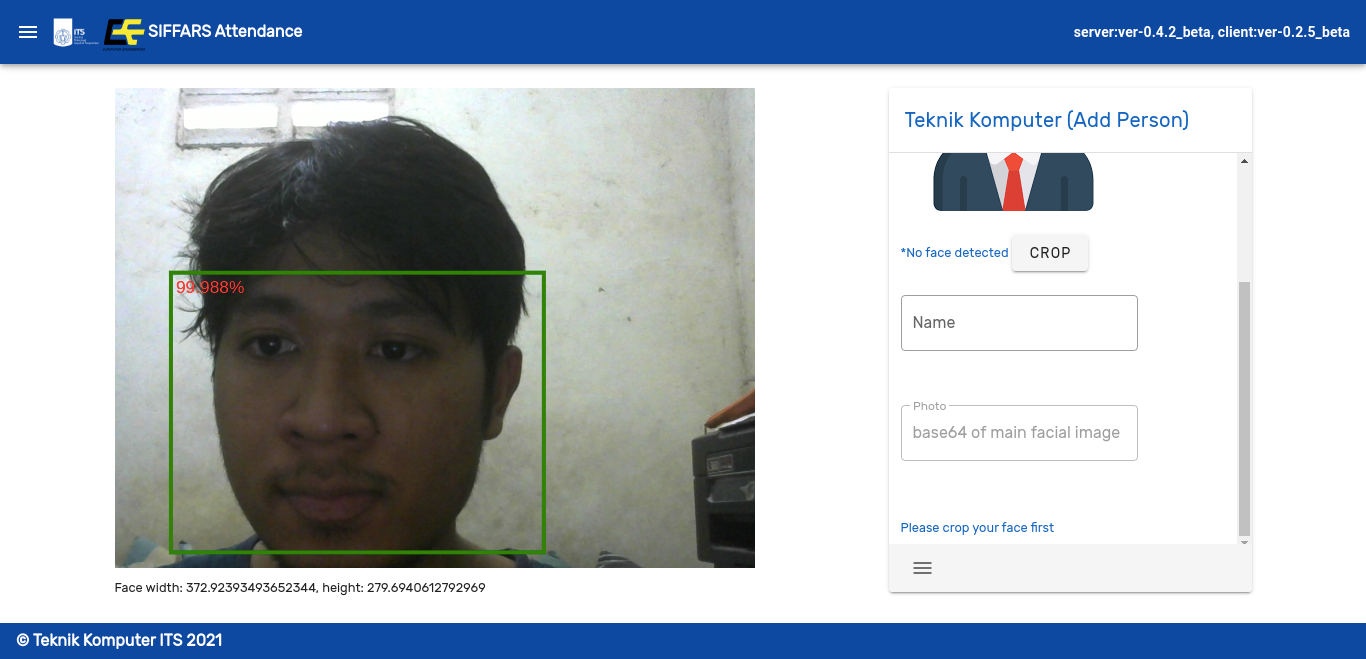
\includegraphics[scale=0.2]{gambar/addpersonfix.png}
  \caption{Page admin untuk menambah data wajah pegawai}
  \label{fig:SfAddperson}

  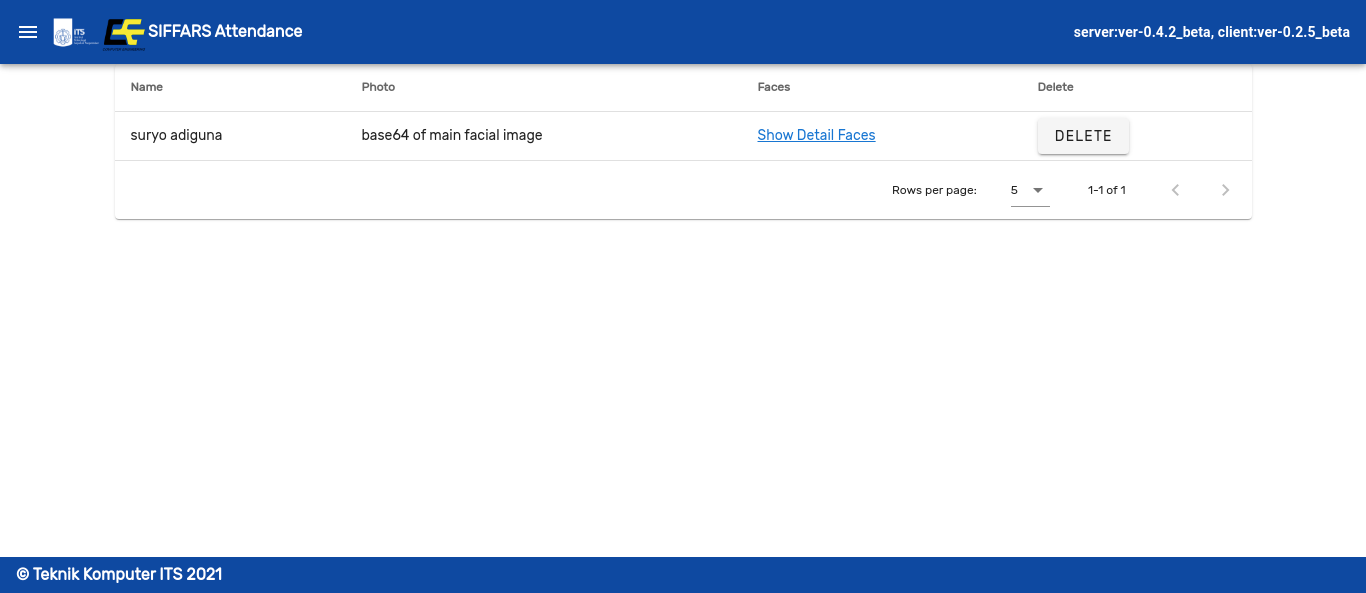
\includegraphics[scale=0.2]{gambar/listperson.png}
  \caption{Page admin untuk melihat data wajah pegawai}
  \label{fig:SfListperson}

  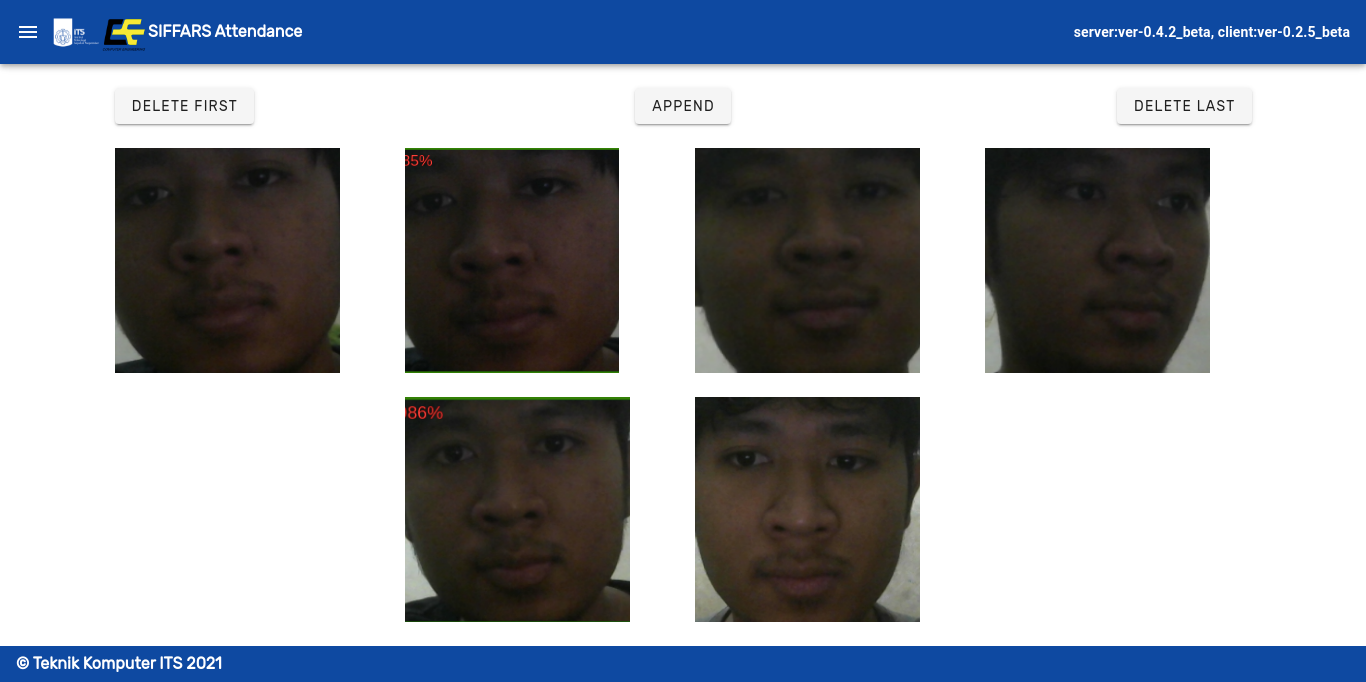
\includegraphics[scale=0.2]{gambar/listface.png}
  \caption{Page admin untuk melihat data wajah tiap pegawai}
  \label{fig:SfListperson}
\end{figure}

\begin{figure} [p] \centering
  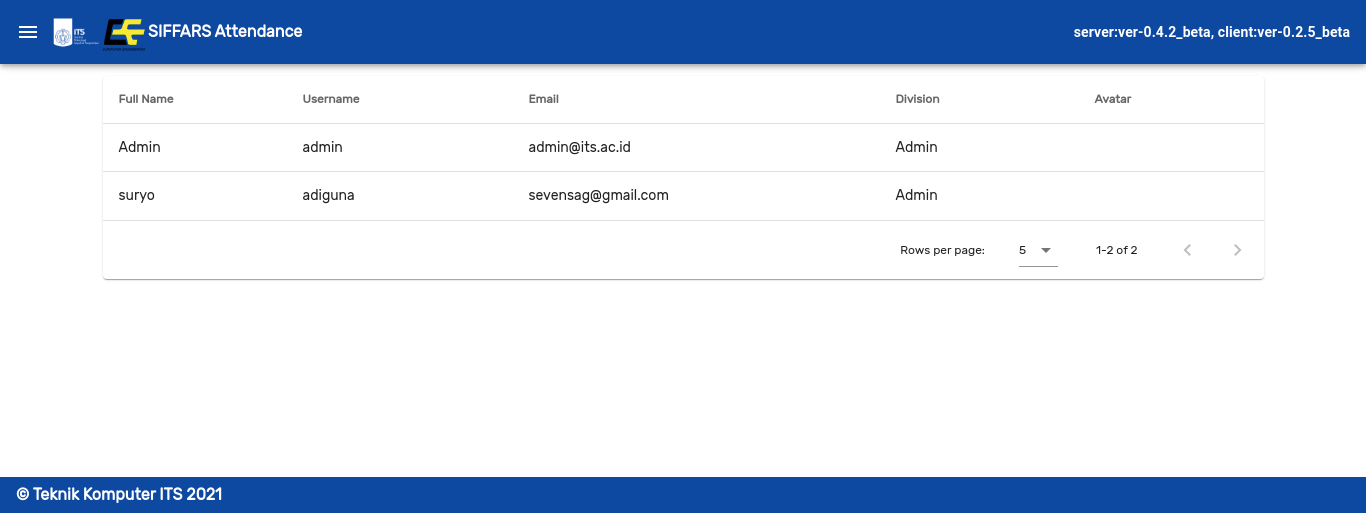
\includegraphics[scale=0.2]{gambar/listuser.png}
  \caption{Page admin untuk melihat data user yang bisa mengakses web siffars}
  \label{fig:SfListperson}

  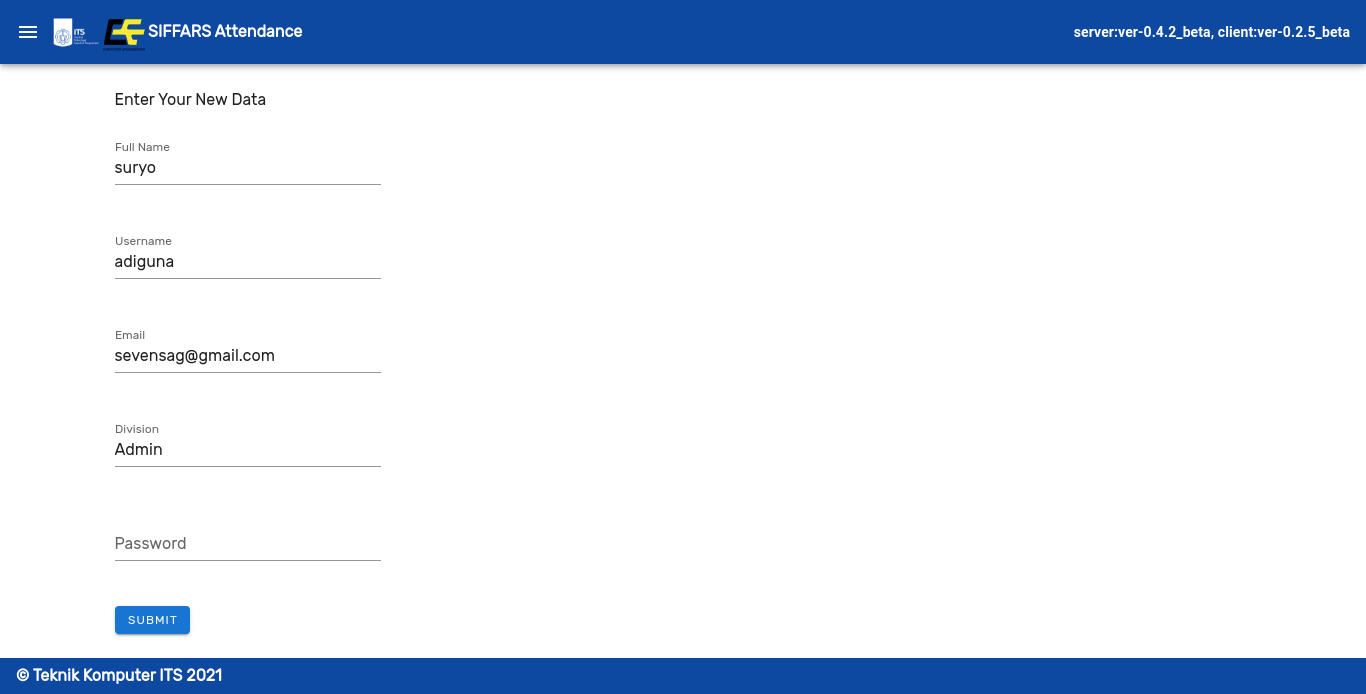
\includegraphics[scale=0.2]{gambar/editaccount.png}
  \caption{Page admin untuk mengedit akun}
  \label{fig:SfListperson}

  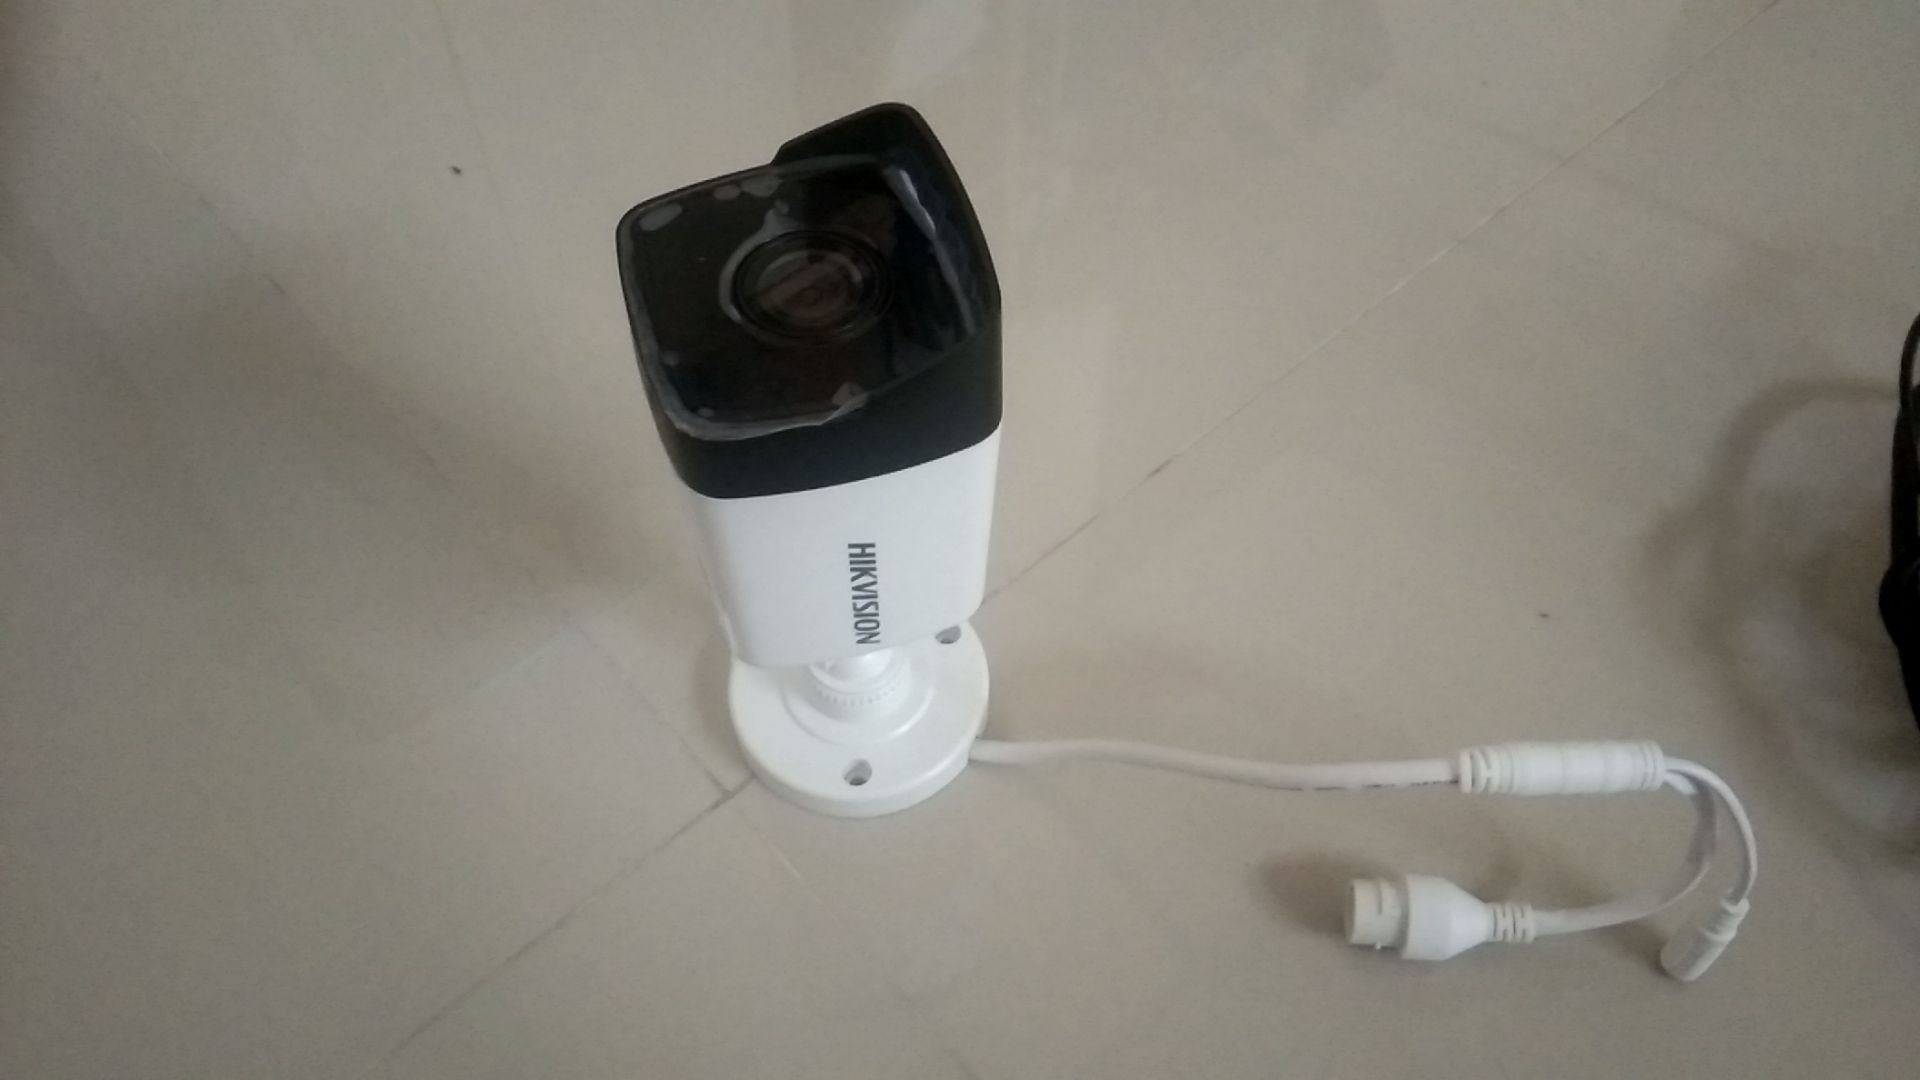
\includegraphics[scale=0.1]{gambar/cctvcctv.jpg}
  \caption{CCTV yang digunakan dalam KP}
  \label{fig:cctv}
\end{figure}

\begin{figure} [p] \centering  
  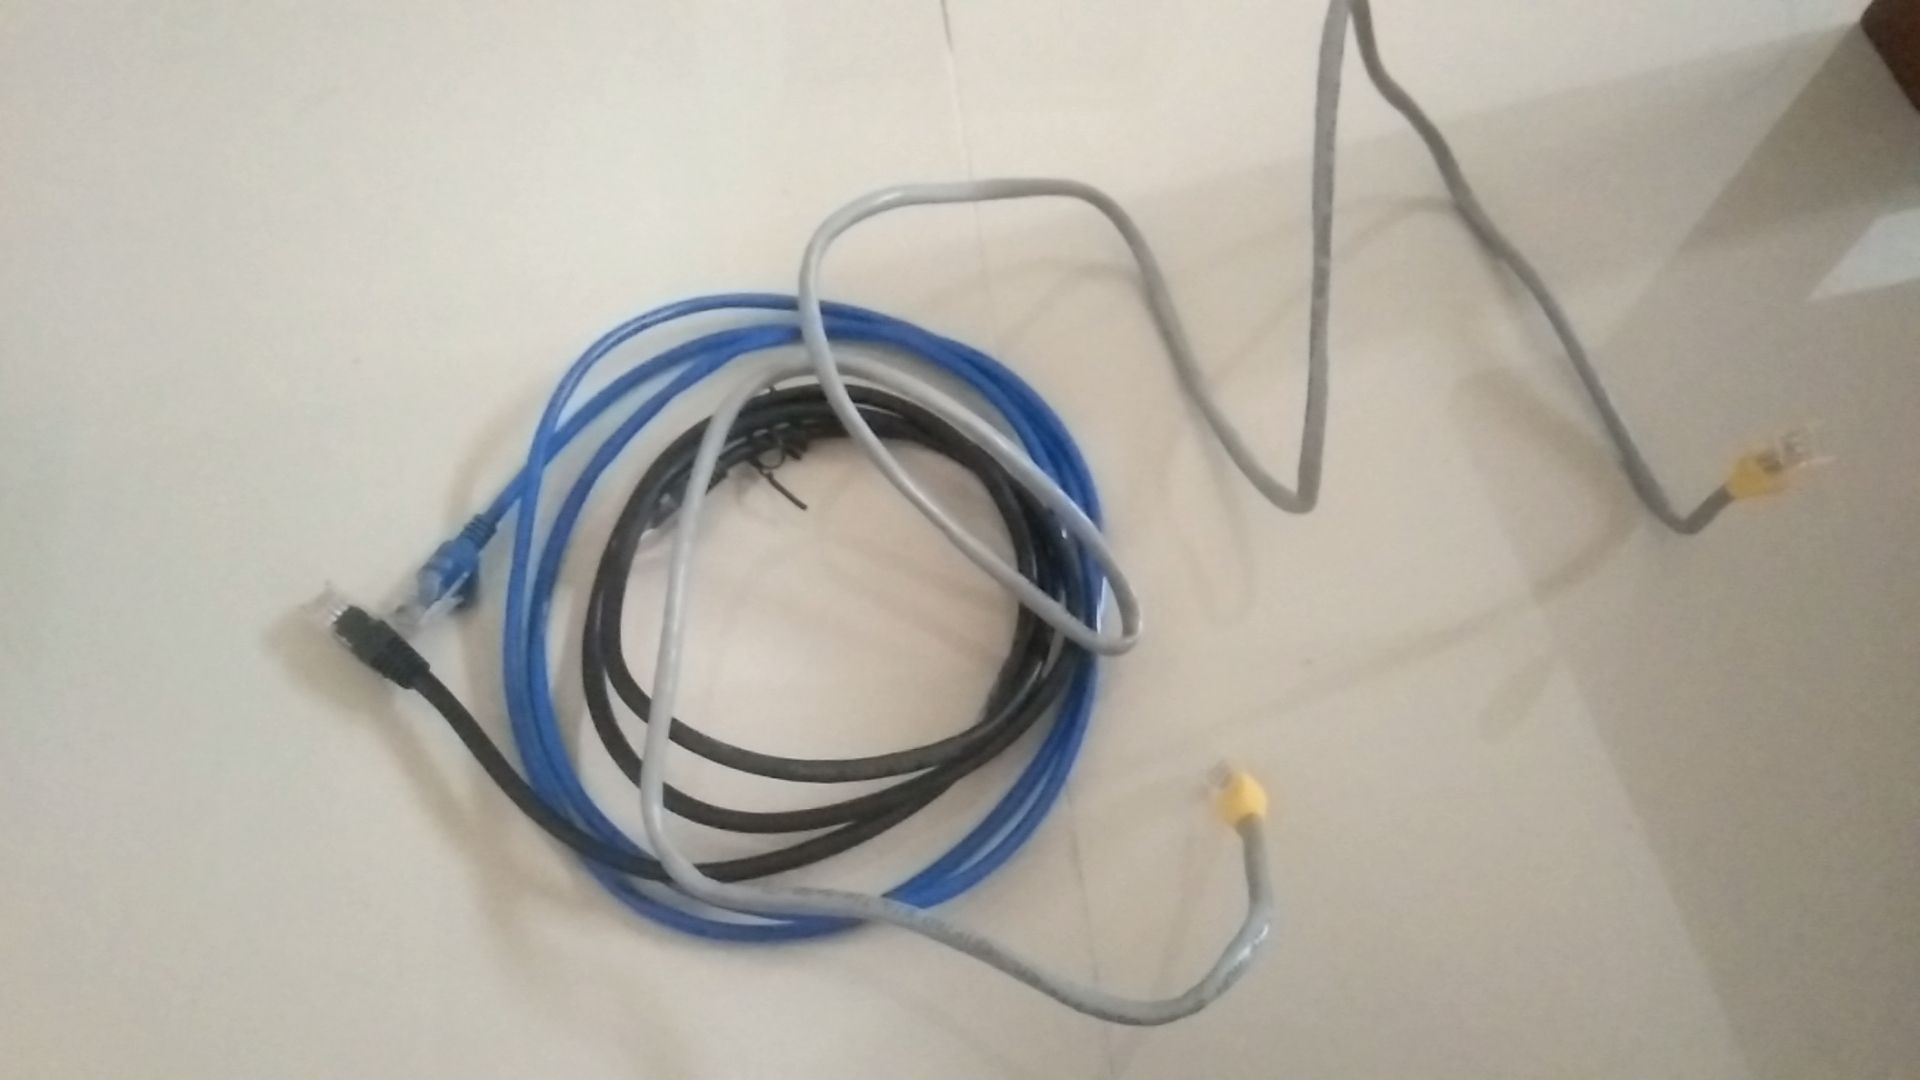
\includegraphics[scale=0.1]{gambar/cctvkabellan.jpg}
  \caption{Kabel lan RJ45}
  \label{fig:kabellan}

  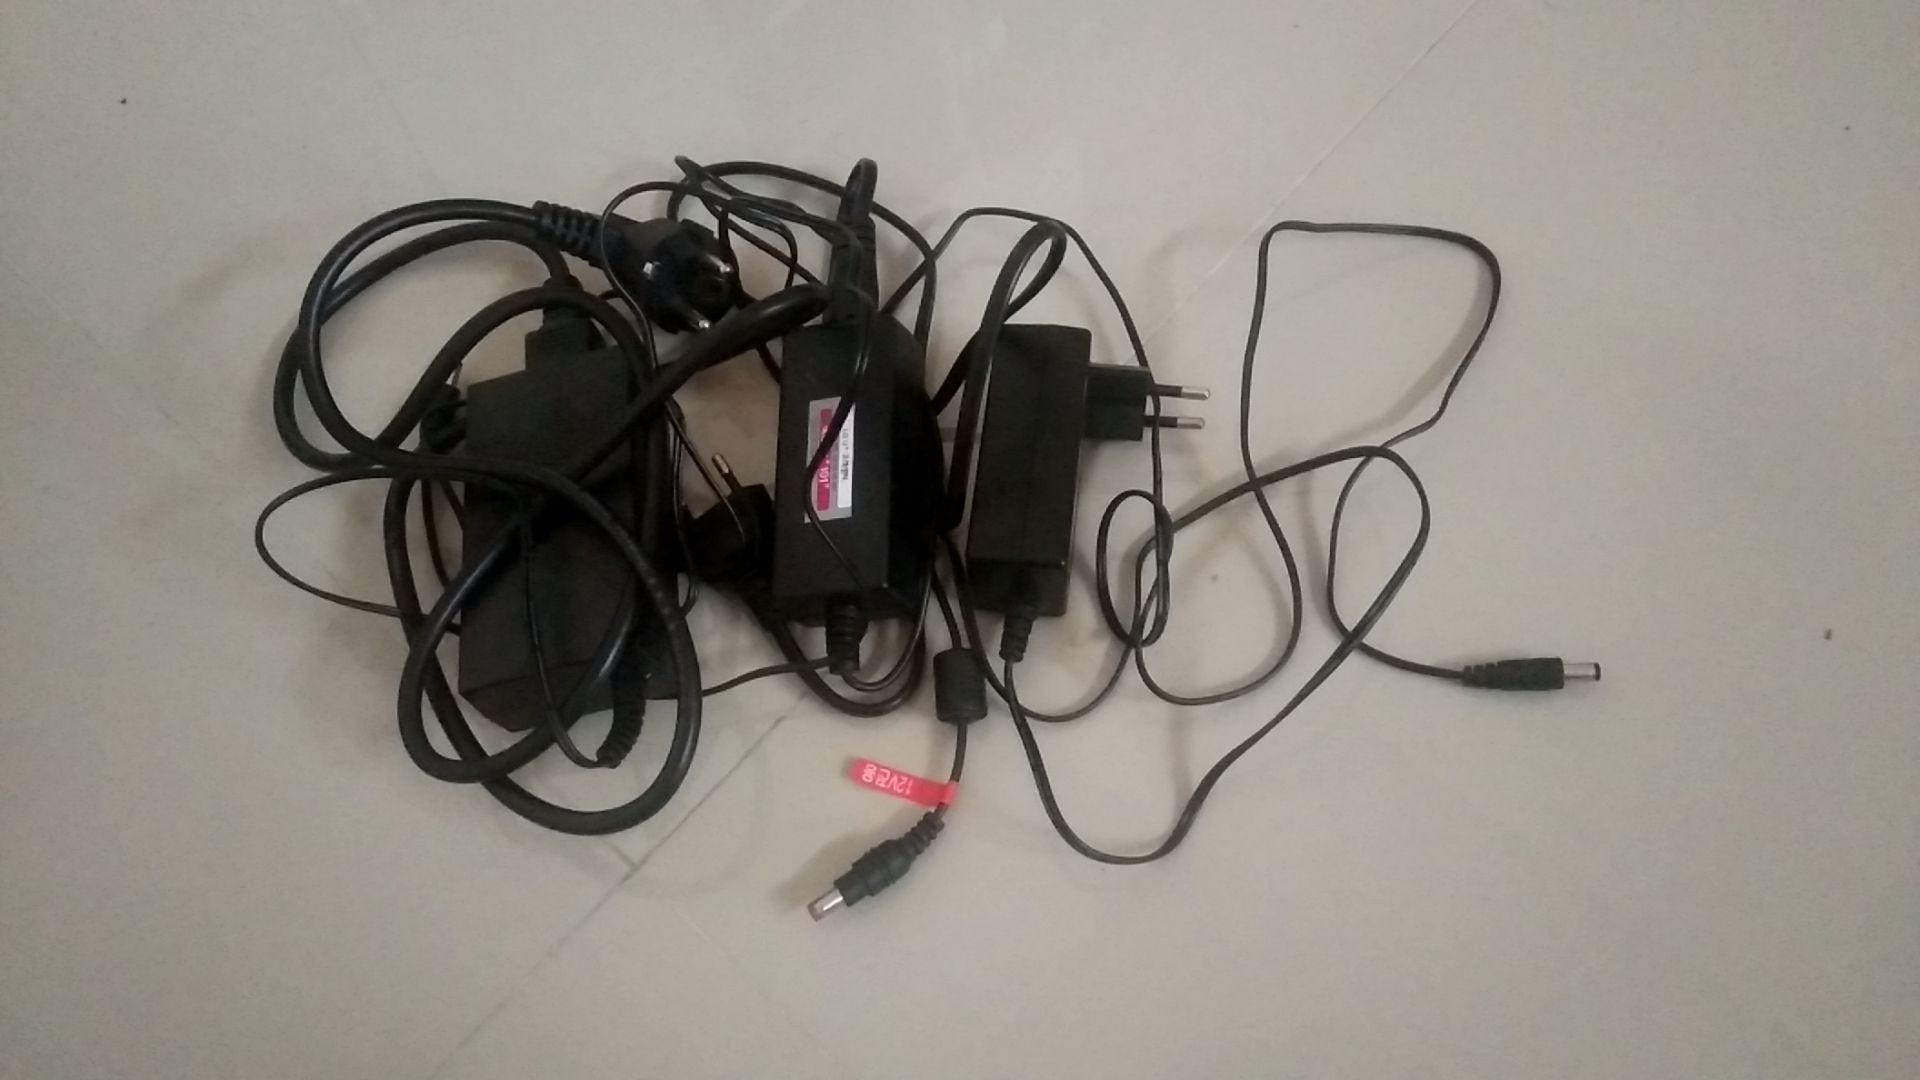
\includegraphics[scale=0.1]{gambar/cctvadapter.jpg}
  \caption{Adaptor untuk switch, nvr, dan CCTV}
  \label{fig:adapter}

  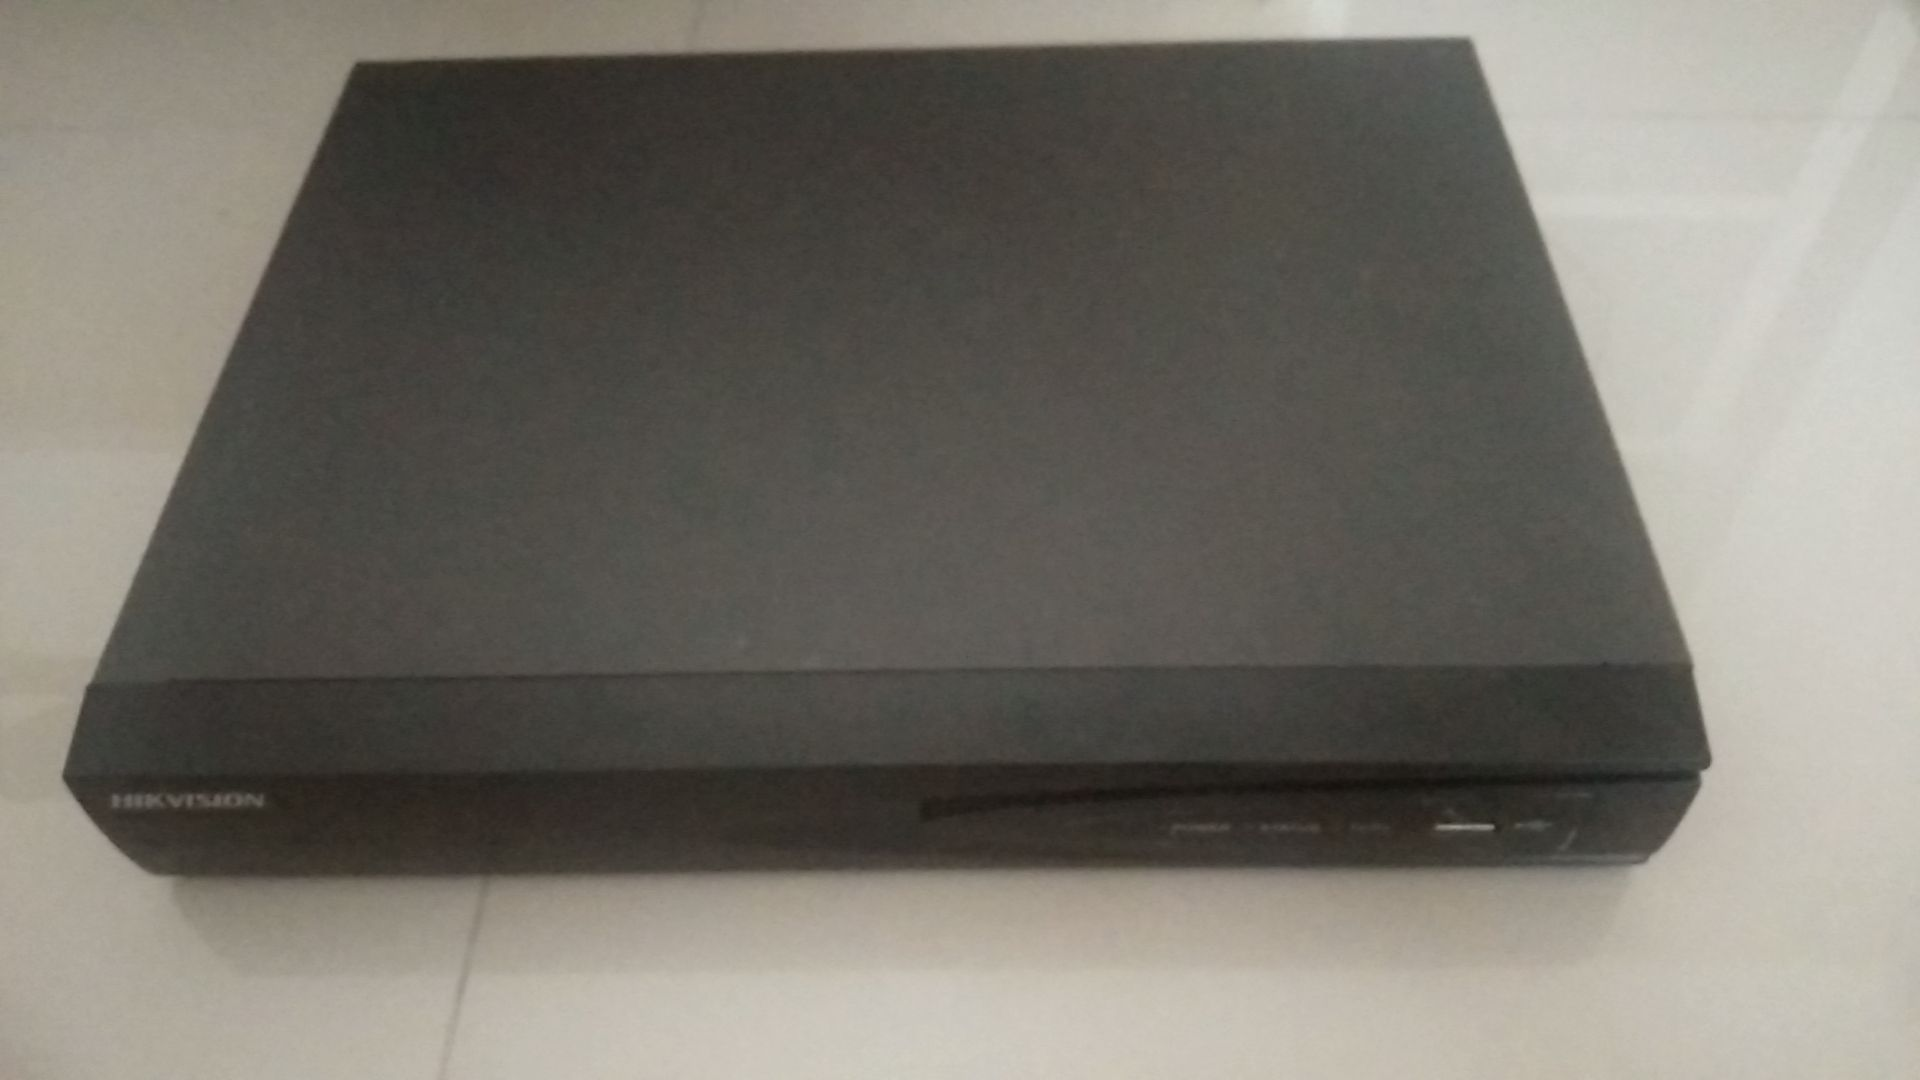
\includegraphics[scale=0.1]{gambar/cctvnvr.jpg}
  \caption{NVR}
  \label{fig:nvr}

\end{figure}

\begin{figure} [p] \centering  
  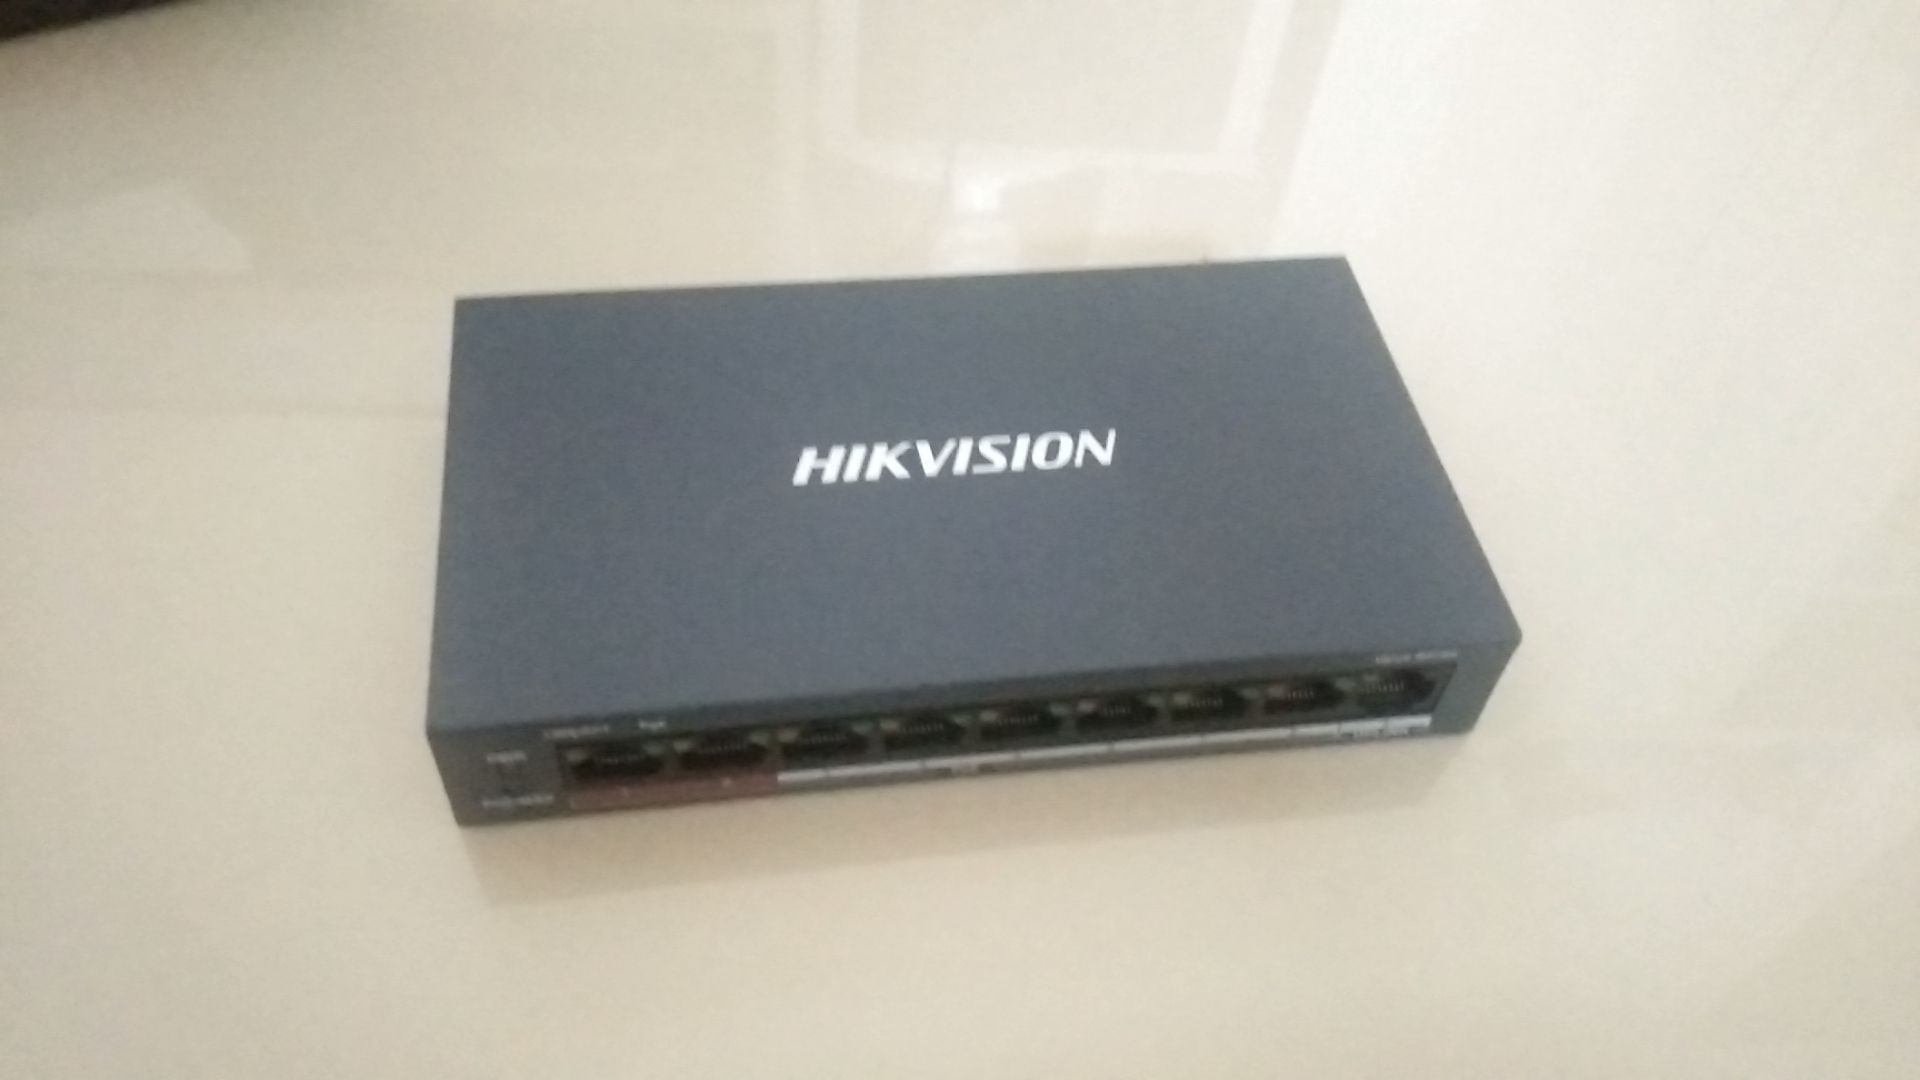
\includegraphics[scale=0.1]{gambar/cctvswitch.jpg}
  \caption{Switch}
  \label{fig:switch}

  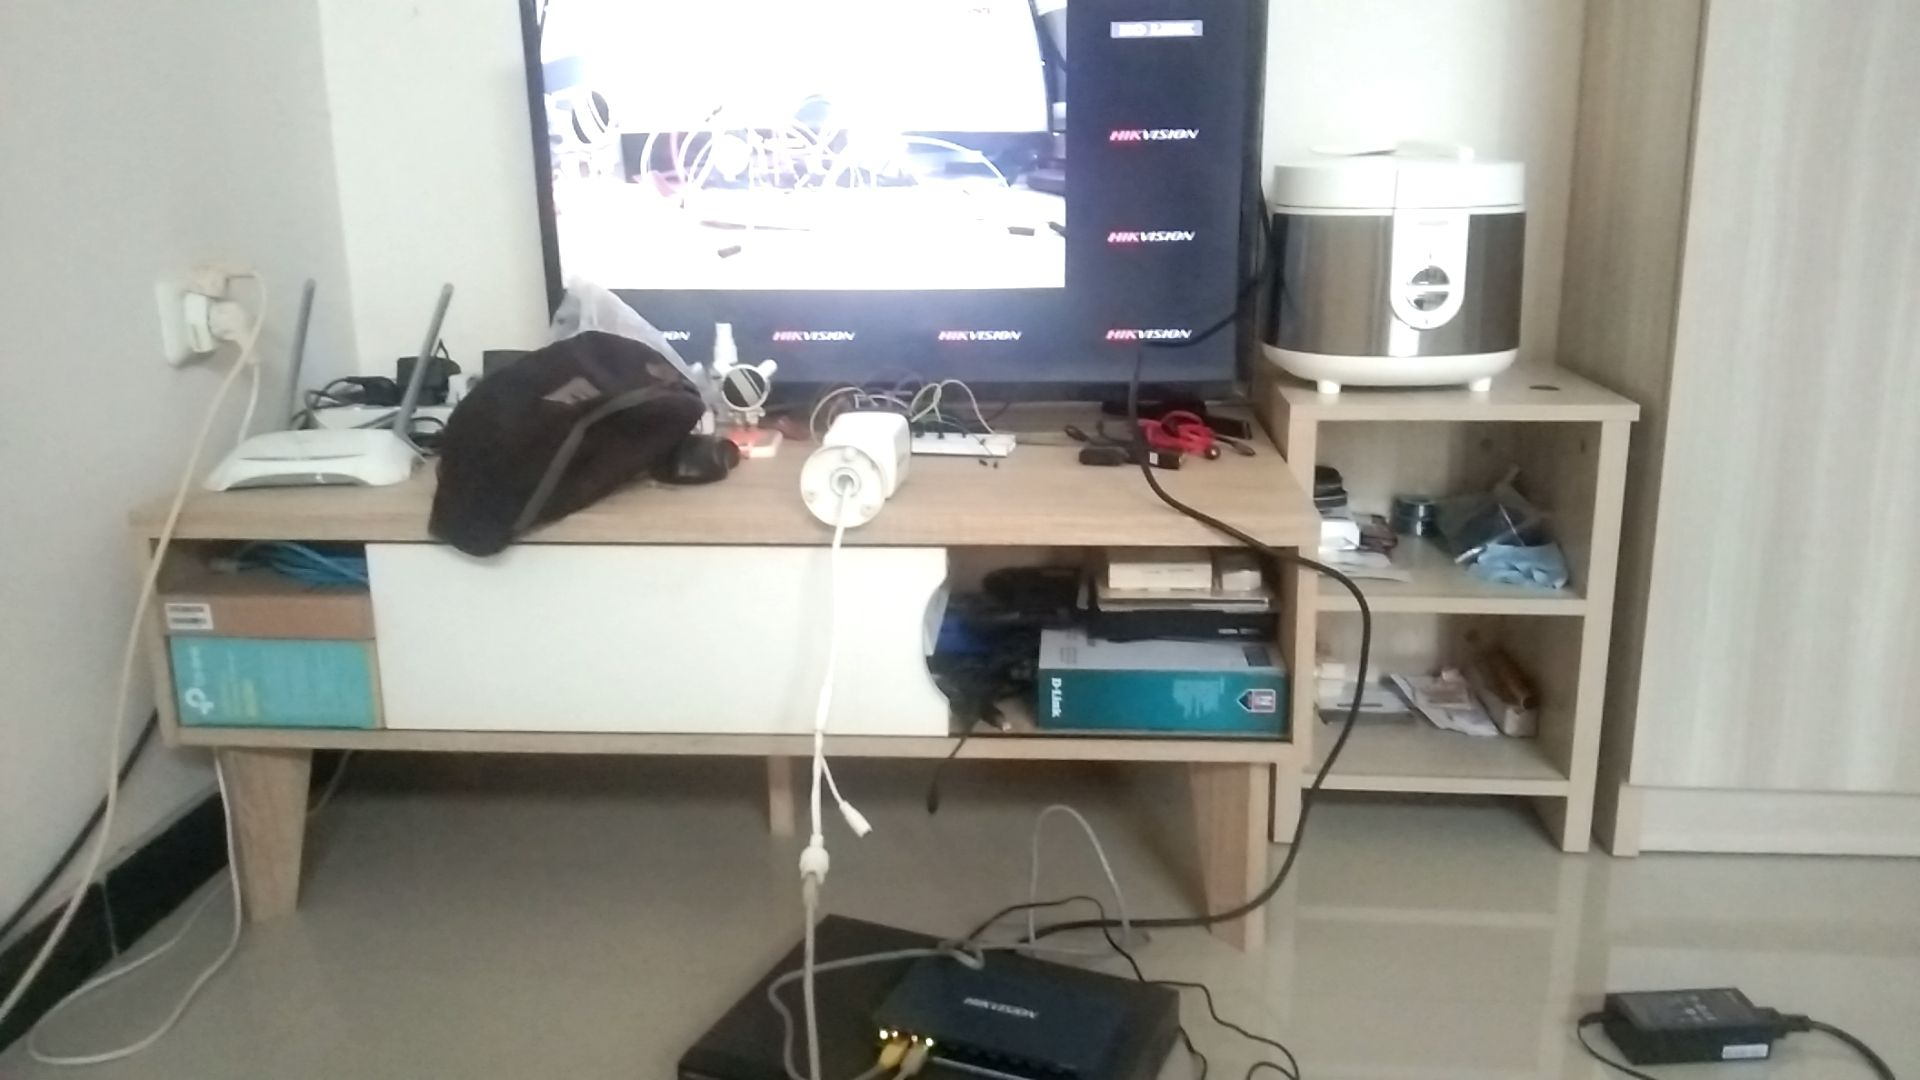
\includegraphics[scale=0.1]{gambar/cctvfullsistem.jpg}
  \caption{Full sistem CCTV yang telah terpasang}
  \label{fig:fullsistemcctv}
\end{figure}

% Contoh pembuatan code snippet
% \begin{lstlisting}[
%   language=C++,
%   label={lst:Hello World},
%   caption={Program hello world}
% ]
% #include <iostream>

% int main() {
%     std::cout << "Hello World!";
%     return 0;
% }
% \end{lstlisting}

% % Contoh penggunaan referensi dari code snippet yang diinputkan
% Seperti contoh pada baris program Listing \ref{lst:Hello World} dan Listing \ref{lst:PrimeNumber}, \lipsum[23]

% % Contoh input code snippet
% \lstinputlisting[
%   % Bahasa yang digunakan oleh code snippet
%   language=Python,
%   % Label referensi dari code snippet yang diinputkan
%   label={lst:PrimeNumber},
%   % Keterangan dari code snippet yang diinputkan
%   caption={Program perhitungan bilangan prima}
% % Nama dari file code snippet yang diinputkan
% ]{program/prime-number.py}
